\documentclass[a4paper,11pt]{article}

\usepackage[left=2cm,text={17cm, 24cm},top=3cm]{geometry}

\usepackage[utf8]{inputenc}
\usepackage[czech]{babel}
\usepackage[IL2]{fontenc}

\usepackage{times, picture, graphics}
 
\usepackage[linesnumbered,ruled,vlined]{algorithm2e}
\SetAlgorithmName{Algoritmus}{algoritmus}

% balicky pro odkazy
\usepackage{url}

\hyphenation{symbolem}

\pagenumbering{arabic}

\begin{document}

\begin{titlepage}
\begin{center}
\fontsize{27.1}{20}\selectfont\textsc{{Vysoké učení technické v~Brně}}\\
\vspace{\stretch{0.0075}}
\fontsize{22.7}{0}\textsc{\selectfont{Fakulta informačních technologií}}\\
\vspace{\stretch{0.381}}
\LARGE{Typografie a publikování\,--\,3. projekt}\\
\Huge{Tabulky a obrázky}
\vspace{\stretch{0.616}}
\end{center}

{\hspace*{-0.6cm}\Large \today \hfill
Jakub Švestka}

\end{titlepage}

\newpage
\pagestyle{plain}

\section{Úvodní strana}
Název práce umístěte do zlatého řezu a nezapomeňte uvést dnešní datum a vaše jméno a příjmení.

\section{Tabulky}
Pro sázení tabulek můžeme použít buď prostředí\texttt{ tabbing }nebo prostředí\texttt{ tabular}.

\subsection{Prostředí\texttt{ tabbing}}
Při použití\texttt{ tabbing }vypadá tabulka následovně:
\begin{tabbing}\\[-0.55cm]

Vodní melouny \quad \= 25,90 \quad \= Množství \= \kill
\textbf{Ovoce} \> \textbf{Cena} \> \textbf{Množství}\\
Jablka \> 25,90 \> 3\ kg\\
Hrušky \> 27,40 \> 2,5\ kg\\
Vodní melouny \> 35,-- \> 1\ kus\\
\end{tabbing}

\noindent Toto prostředí se dá také použít pro sázení algoritmů, ovšem vhodnější je použít prostředí\texttt{ algorithm }nebo\texttt{ algorithm2e }(viz sekce \ref{sekce3}).

\subsection{Prostředí\texttt{ tabular}} 
Další monžostí, jak vytvořit tabulku, je použít prostředí\texttt{ tabular}. Tabulky pak budou vypadat takto\footnote{Kdyby byl problem s\texttt{ cline, }zkuste se podívat třeba sem: http://www.abclinuxu.cz/tex/poradna/show/325037.}:
\bigskip
\begin{table}[h]
\catcode`\-=12
  \begin{center}
    \begin{tabular}{| l | r | r |}
    \hline  
      & \multicolumn{2}{| c |}{\textbf{Cena}} \\ \cline{2-3}
      \textbf{Měna} & \textbf{nákup} & \textbf{prodej} \\ \hline 
      EUR & 24,501 & 24,324 \\
      JPY & 105,484 & 105,847 \\
      USD & 16,632 & 16,328 \\
    \hline
  \end{tabular}
    \caption{Tabulka kurzů k~dnešnímu dni}
    \label{tabulka1}
  \end{center}
\end{table}



\begin{table}[h]
\catcode`\-=12
  \begin{center}
   \begin{tabular}{| c | c |}
     \hline
       $A$ & $\neg A$ \\ \hline
       \textbf{P} & N \\ \hline
       \textbf{X} & X \\ \hline
       \textbf{N} & P \\
     \hline
   \end{tabular}   
   \begin{tabular}{| c | c | c | c | c |} 
     \hline 
      \multicolumn{2}{| c |}{} & \multicolumn{3}{| c |}{$B$} \\ \cline{3-5}
      \multicolumn{2}{| c |}{$A \vee B$} & \textbf{P} & \textbf{X} & \textbf{N} \\ \hline
      \multicolumn{1}{| c |}{} & \textbf{P} & P & P & P \\ \cline{2-5}
                           $A$ & \textbf{X} & P & X & X \\ \cline{2-5}
      \multicolumn{1}{| c |}{} & \textbf{N} & P & X & N \\
     \hline
   \end{tabular}
   \begin{tabular}{| c | c | c | c | c |} 
     \hline 
      \multicolumn{2}{| c |}{} & \multicolumn{3}{| c |}{$B$} \\ \cline{3-5}
      \multicolumn{2}{| c |}{$A \wedge B$} & \textbf{P} & \textbf{X} & \textbf{N} \\ \hline
      \multicolumn{1}{| c |}{} & \textbf{P} & P & X & N \\ \cline{2-5}
                           $A$ & \textbf{X} & X & X & N \\ \cline{2-5}
      \multicolumn{1}{| c |}{} & \textbf{N} & N & N & N \\
     \hline
   \end{tabular}
   \begin{tabular}{| c | c | c | c | c |} 
     \hline 
      \multicolumn{2}{| c |}{} & \multicolumn{3}{| c |}{$B$} \\ \cline{3-5}
      \multicolumn{2}{| c |}{$A \rightarrow B$} & \textbf{P} & \textbf{X} & \textbf{N} \\ \hline
      \multicolumn{1}{| c |}{} & \textbf{P} & P & X & N \\ \cline{2-5}
                           $A$ & \textbf{X} & P & X & X \\ \cline{2-5}
      \multicolumn{1}{| c |}{} & \textbf{N} & P & P & P \\
     \hline
   \end{tabular}      
    \caption{Kleeneho trojhodnotová logika}
    \label{tabulka2}
  \end{center}
\end{table}


\section{Algoritmy}\label{sekce3}
Pokud budeme chtít vysázet algoritmus, můžeme použít prostředí\texttt{ algorithm\footnote{Pro\,nápovědu,\,jak\,zacházet\,s~prostředím\texttt{ algorithm, }můžeme\,zkusit\,tuhle\,stránku:\\ http://ftp.cstug.cz/pub/tex/CTAN/macros/latex/contrib/algorithms/algorithms.pdf.} } nebo\texttt{ algorithm2e}\footnote{Pro\texttt{ algorithm2e }zase tuhle: http://ftp.cstug.cz/pub/tex/CTAN/macros/latex/contrib/algorithm2e/algorithm2e.pdf.}.\\
Příklad použití prostředí\texttt{ algorithm2e }viz Algoritmus \ref{algoritmus}.
\newpage
\vspace*{-0.15cm}
\IncMargin{1.2em}
\begin{algorithm}
  \SetAlgoNoLine
  \SetNlSkip{0em}
  \SetNlSty{normal}{}{:}
  \SetKwInput{Input}{Input}
  \SetKwInOut{Output}{Output}
  \SetKwFor{For}{for}{do}{end\,for}
\Indm  
    \Input{$(X_{t-1},u_t,z_t)$}
    \Output{$X_t$} 
\Indp
\Indp
  \BlankLine
  $\overline{X_t} = X_t = 0$ \BlankLine   
  \For{$k = 1$ to $M$}{   
    $x_t^{[k]} = sample\_motion\_model(u_t, x_{t-1}^{[k]})$\\
    $\omega_t^{[k]} = measuremen\_model(z_t, x_{t}^{[k]}, m_{t-1}^{[k]})$\\
    $m_t^{[k]} = updated\_occupancy\_grid(z_t, x_{t}^{[k]}, m_{t-1}^{[k]})$\\
    $\overline{X_t} = \overline{X_t} + \langle x_x^{[m]},\omega_t^{[m]} \rangle $
  }
  
  \For{$k = 1$ to $M$}{   
    draw $i$ with probability $\approx \omega_t^{[i]}$\\
    add $\langle x_x^{[k]},m_t^{[k]} \rangle$ to $X_t$
  }
  \Return{$X_t$}
        
\caption{\textsc{Fast}SLAM\label{algoritmus}}
\end{algorithm}
\DecMargin{1.2em}

\section{Obrázky}
Do našich článku můžeme samozřejmě vkládat obrázky. Pokud je obrázkem fotografie, m;žeme klidně použít bitmapový soubor. Pokud by to ale mělo být nějaké schéma nebo něco podobného, je dobrým zvykem takovýto obrázek vytvořit vektorově.

\begin{figure}[ht]
  \begin{center}
    \scalebox{0.4}{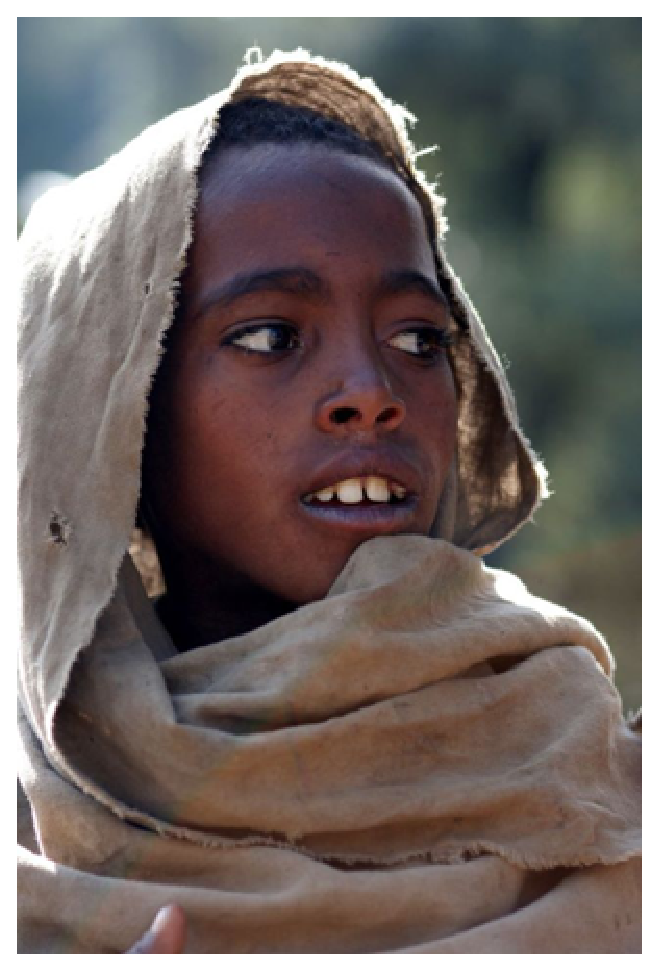
\includegraphics{etiopan.eps}
    \reflectbox{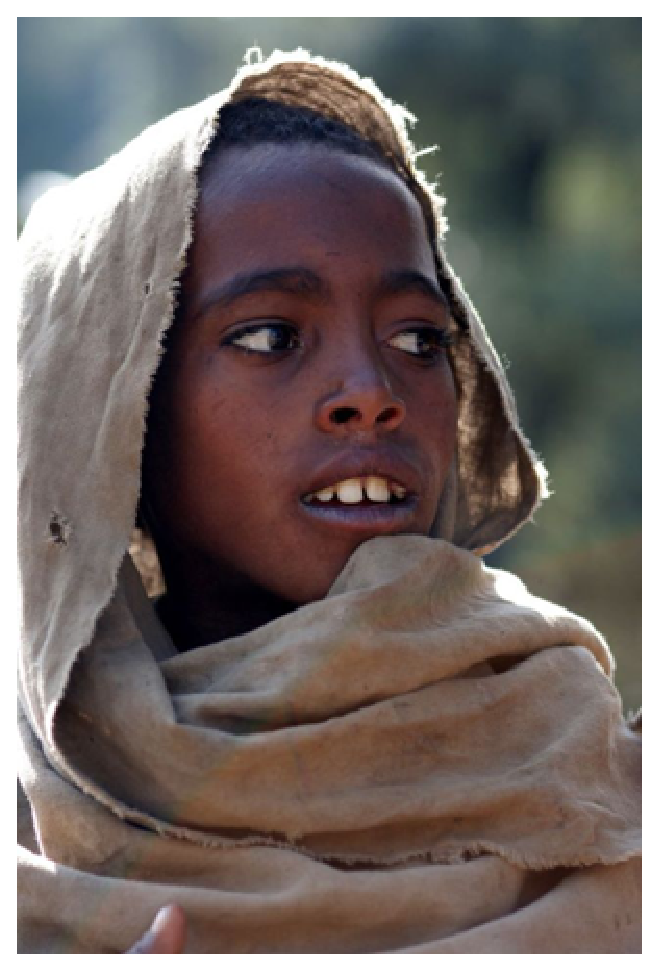
\includegraphics{etiopan.eps}} }
    \caption{Malý etiopánek a jeho bratříček}
    \label{etiopan}
  \end{center}
\end{figure}

\newpage

Rozdíl mezi vektorovým\,\ldots
\begin{figure}[ht]
  \begin{center}
    \scalebox{0.4}{
\includegraphics{oniisan.eps}}
    \caption{Vektorový obrázek}
    \label{vektorovy}
  \end{center}
\end{figure}


\noindent\ldots\,a bitmapovým obrázkem
\begin{figure}[ht]
  \begin{center}
    \scalebox{0.6}{
\includegraphics{oniisan2.eps}}
    \caption{Bitmapový obrázek}
    \label{bitmapovy}
  \end{center}
\end{figure}

se projeví například při zvětšení.

Odkazy (nejen ty) na obrázky \ref{etiopan}, \ref{vektorovy}, \ref{bitmapovy}, na tabulky \ref{tabulka1} a \ref{tabulka2}
a také algoritmus \ref{algoritmus} jsou udělány pomocí křižových odkazů.
Pak je ovšem potřeba zdrojový soubor přeložit dvakrát.

Vektorové obárzky lze vytvořit i přímo v~{\LaTeX}u, například pomocí prostředí\,\,\texttt{picture. }Všechny rozměry jsou uváděny v~mm.




\newpage

\begin{figure}
\begin{center}
\setlength{\unitlength}{1.35mm}
\begin{picture}(115,158.5)

%ohraničení stránky
\put(0,0){\linethickness{1pt}\framebox(115,158.5){}}

%pravá strana
  \put(91,145){\makebox(15,14.5){\shortstack{Výška \\ mezery\,=\,14,5}}}
  \put(88,151.25){\vector(0,1){7.25}}
  \put(88,151.25){\vector(0,-1){7.25}}
  
  \put(89,132){\makebox(15,14.5){\shortstack{Výška \\ mezery\,=\,10}}}
  \put(88,139){\vector(0,1){5}}
  \put(88,139){\vector(0,-1){5}}
  
  \put(90,122){\makebox(15,14.5){\shortstack{Výška \\ hlavičky\,=\,10}}}
  \put(88,129){\vector(0,1){5}}
  \put(88,129){\vector(0,-1){5}}
  
  \put(89,110){\makebox(15,14.5){\shortstack{Výška \\ mezery\,=\,14}}}
  \put(88,117){\vector(0,1){7}}
  \put(88,117){\vector(0,-1){7}}
  
  %poznámka
  \put(94,77.5){\linethickness{1pt}\framebox(15,10){\textbf{\shortstack{Okrajová\\ poznámka}}}}
  \put(92,88){\makebox(20,14.5){\shortstack{Šířka\\ boxu\,=\,15}}}
  \put(102,91.5){\vector(-1,0){7.5}}
  \put(102,91.5){\vector(1,0){7.5}}
  \put(87.5,97.5){\makebox(20,14.5){\shortstack{Mezera\,=\,9}}}
  \put(94,103.5){\vector(-1,-3){4}}
  \put(90,91.5){\vector(-1,0){4.5}}
  \put(90,91.5){\vector(1,0){4.5}}
  
  %pokračujeme pod poznámkou
  \put(87.5,57){\makebox(15,14.5){\shortstack{Výška\\ těla\,=\,75}}}
  \put(88,72.5){\vector(0,1){37.5}}
  \put(88,72.5){\vector(0,-1){37.5}}
  
  \put(89.5,19){\makebox(15,14.5){\shortstack{Výška\\ mezery\,=\,15}}}
  \put(88,27.5){\vector(0,1){7.5}}
  \put(88,27.5){\vector(0,-1){7.5}}
  
  \put(88,6){\makebox(15,14.5){\shortstack{Výška\\ paty\,=\,10}}}
  \put(88,15){\vector(0,1){5}}
  \put(88,15){\vector(0,-1){5}}  

%rozměry stránky
  %šířka = 115
  \put(53,3){\makebox(10,5){\shortstack{Šířka stránky = 115}}}
  \put(57.5,3){\vector(1,0){57.5}}
  \put(57.5,3){\vector(-1,0){57.5}}
  %výška = 158,5 (popis ke kótě)
  \put(94,43){\makebox(15,14.5){\shortstack{Výška\\ stránky\,=\,158,5}}}
  \put(102,55){\vector(1,1){10}}
  %kóta
  \put(112,79.25){\vector(0,1){79.25}}
  \put(112,79.25){\vector(0,-1){79.25}}

%čárkované čáry
  \multiput(15,151.5)(0,-10){16}{\line(0,1){7}}
  \multiput(0,144)(10,0){11}{\line(1,0){7}}   

%levá strana
  \put(2.5,91.5){\makebox(10,5){\shortstack{Mezera = 15}}}
  \put(7.5,91.5){\vector(1,0){7.5}}
  \put(7.5,91.5){\vector(-1,0){7.5}}

%box hlavička
  \put(53,137){\makebox(10,5){\shortstack{Šířka boxu = 55}}}
  \put(57.5,137){\vector(1,0){27.5}}
  \put(57.5,137){\vector(-1,0){27.5}}
  \put(30,124){\linethickness{1pt}\framebox(55,10){\textbf{Hlavička}}}

%box tělo
  \put(30,35){\linethickness{1pt}\framebox(55,75){\textbf{Textové tělo}}}
%box pata
  \put(30.5,10){\linethickness{1pt}\framebox(55,10){\textbf{Pata}}}
  \end{picture}

\caption{Vektorový obrázek v~prostředí \texttt{picture}}
\end{center}
\end{figure}
\end{document} 